\documentclass{article}

\usepackage{listings}
\usepackage{url}
\usepackage{hyperref}
\usepackage{graphicx}
\usepackage{xepersian}
\usepackage{ulem}


\settextfont{XB Zar}
\setlatintextfont{XB Zar}


\makeatletter
\let\@@scshape=\scshape
\renewcommand{\scshape}{%
  \ifnum\strcmp{\f@series}{bx}=\z@
    \usefont{T1}{cmr}{bx}{sc}%
  \else
    \ifnum\strcmp{\f@shape}{it}=\z@
      \fontshape{scsl}\selectfont
    \else
      \@@scshape
    \fi
  \fi}
\makeatother

\title{
مستند فاز اول پروژه
\\
\vspace{4mm}
سیستم‌های عامل
\\
\vspace{2mm}
دکتر جلیلی
}

\author{
محمدحسین اعلمی
\hspace{1cm}
۹۴۱۰۴۴۰۱
\\
محمدمهدی فاریابی
\hspace{1cm}
۹۳۱۰۱۹۵۱
}

\date{}
\begin{document}

\maketitle

\section*{مقدمه}
این مستند گزارش انجام فاز اول پروژه درس سیستم‌های عامل به منظور آشنایی با کرنل لینوکس و سیستم‌عامل اندروید است. تمامی عملیات‌های ذکر‌شده در مستند روی سیستم‌عامل
\lr{Ubuntu 16.04}
پیاده و تست‌ شده‌اند.

\section*{نصب شبیه‌ساز QEMU}
همان‌طور که در صورت پروژه نیز ذکر شده است، ما از شبیه‌ساز\footnote{\lr{Emulator}} QEMU \cite{1} به منظور شبیه‌سازی محیط اندروید روی سیستم‌عامل لینوکس استفاده می‌کنیم. به منظور نصب QEMU دستور زیر را در ترمینال اجرا می‌کنیم:

\begin{latin}
\begin{verbatim}
$ sudo apt-get install qemu qemu-kvm
\end{verbatim}
\end{latin}

\section*{دریافت فایل تصویر ایزوی اندروید}
فایل تصویر ایزوی
\lr{Android-x86} 
را از 
\href{http://www.android-x86.org/}{سایت مرجع آن}
 دریافت می‌کنیم.
 
\section*{ساختن درایو مجازی}
در ادامه بایستی یک درایو مجازی\footnote{\lr{Virtual Drive}} بسازیم تا سیستم‌عامل اندروید را روی آن بوت کنیم. به این منظور بایستی از فایل ایزوی دانلود شده و QEMU استفاده کنیم. ابتدا فایل ایزو را به دایرکتوری مد نظرمان منتقل می‌کنیم:

\begin{latin}
\begin{verbatim}
$ mv ~/Downloads/android-x86_64-7.1-rc2.iso ~/Desktop/OS\ Project/
\end{verbatim}
\end{latin}

سپس درایو مجازی‌مان را با دستور زیر می‌سازیم:

\begin{latin}
\begin{verbatim}
$ qemu-img create -f qcow2 android71.qcow2 8G
\end{verbatim}
\end{latin}

این دستور یک درایو مجازی با پسوند \lr{.qcow2} و با اندازه ۸ گیگابایت می‌سازد. خروجی دستور به شکل زیر است:

\begin{latin}
\begin{verbatim}
Formatting 'android71_qcow2.img', fmt=qcow2
size=8589934592 encryption=off cluster_size=65536
lazy_refcounts=off refcount_bits=16
\end{verbatim}
\end{latin}

\section*{بوت کردن و نمایش ماشین مجازی}

حال اکنون دو گزینه داریم، می‌توانیم برای نمایش سیستم اندرویدمان از ابزار VNC\footnote{\lr{Virtual Network Computing}}\cite{2}یا نمایشگر خود Qemu استفاده کنیم. استفاده از VNC این مزیت را دارد که می‌توانیم با فرستادن نمایش ماشین مجازی به یک درگاه، آن را حتی از یک سیستم دیگر و با اتصال به یک درگاه سیستم اجرا کنیم و نیز می‌توانیم از هر ابزار دیگری روی سیستم که قابلیت نمایش VNC را دارد استفاده کنیم، مانند نرم‌افزار‌های کلاینت VNC مانند noVNC \cite{3} یا نرم‌افزار پیش‌فرض ابونتو برای نمایش از راه دور که Vinagre \cite{4} نام دارد.
ما ابتدا از VNC استفاده می‌کنیم تا این مورد را نیز پوشش دهیم.
\\
برای استفاده از ماشین مجازی با VNC دستور زیر را اجرا می‌کنیم:

\begin{latin}
\begin{verbatim}
$ qemu-system-x86_64 \
-display vnc=:5,password -cpu host \
-vga std -enable-kvm -m 4096 \
-usbdevice host:054c:05b9 \
-net nic,macaddr=50:6A:E9:A2:A2:1F,model=rtl8139 \
-monitor telnet:localhost:2350,server,nowait \
-drive file=android71.qcow2,cache=none \
-soundhw es1370 \
-cdrom android-x86_64-7.1-rc2.iso	
\end{verbatim}
\end{latin}

همان‌طور که می‌بینید در خط دوم دستور نمایش این ماشین مجازی به وسیله VNC به درگاه 5905 فرستاده شده است. همین‌طور با توجه به دستور خط ششم روی درگاه 2350 سیستم با Telnet \cite{5} وضعیت Qemu را مانیتور کنیم و تغییراتی روی آن اعمال کنیم،‌ برای مثال پسورد برای دسترسی به ماشین مجازی تعیین کنیم که در ادامه نیز این کار را انجام می‌دهیم. برای این کار این دستور را اجرا می‌کنیم:

\begin{latin}
\begin{verbatim}
$ telnet localhost 2350
Trying 127.0.0.1...
Connected to localhost.
Escape character is '^]'.
QEMU 2.8.1 monitor - type 'help' for more information
(qemu) change vnc password
Password: **********
(qemu) 
telnet> quit
Connection closed.	
\end{verbatim}
\end{latin}

حال می‌توانیم با VNC روی درگاه 5905 با رمزی که در قسمت قبل تعیین کردیم به ماشین مجازی‌مان دسترسی داشته باشیم. برای این کاز از نرم‌افزار Vinagre استفاده می‌کنیم. پس از متصل شدن به درگاه ۵۹۰۵ با VNC و وارد کردن رمز عبور با محیط زیر مواجه می‌شویم(اسکرین‌شات‌های زیر به وسیله نرم‌افزار Vinagre گرفته شده‌اند):

\begin{figure}[ht]
	\centering	
	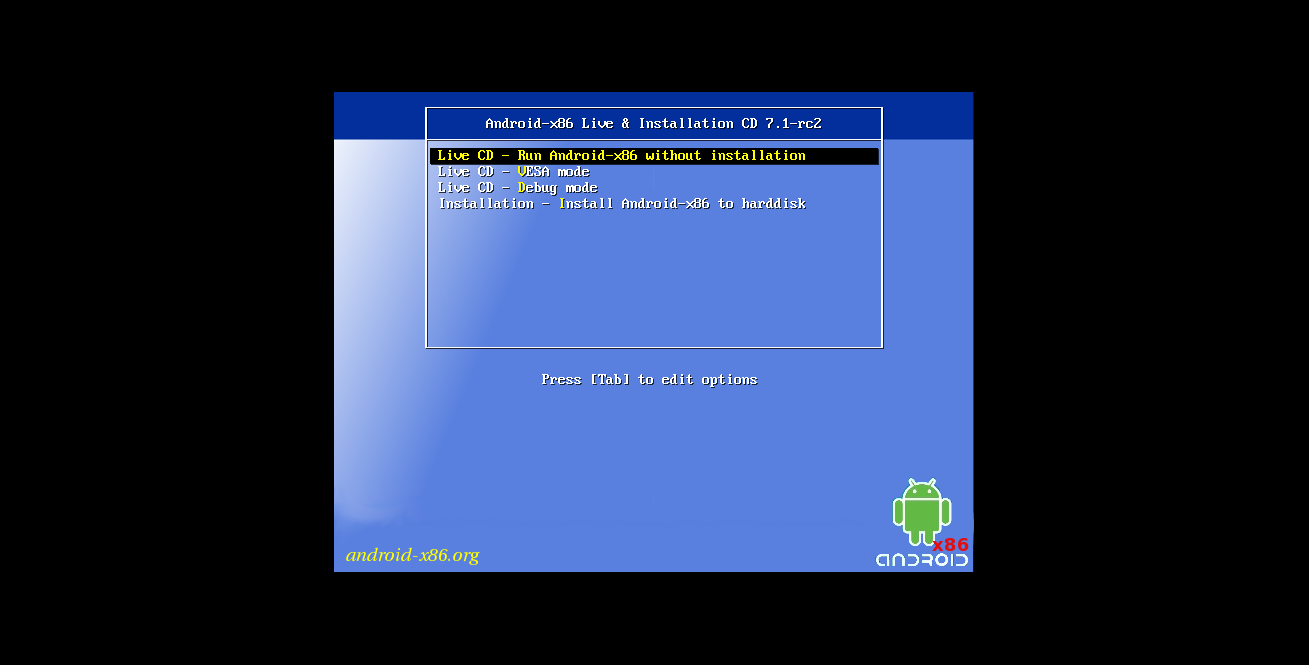
\includegraphics[width = 1\textwidth]{images/install1.png}
\end{figure}

در ادامه مطابق با راهنمای آموزش نصب اندروید روی لینوکس\cite{6} گزینه چهارم یعنی نصب را انتخاب کرده و ادامه می‌دهیم.

\begin{figure}[ht]
	\centering	
	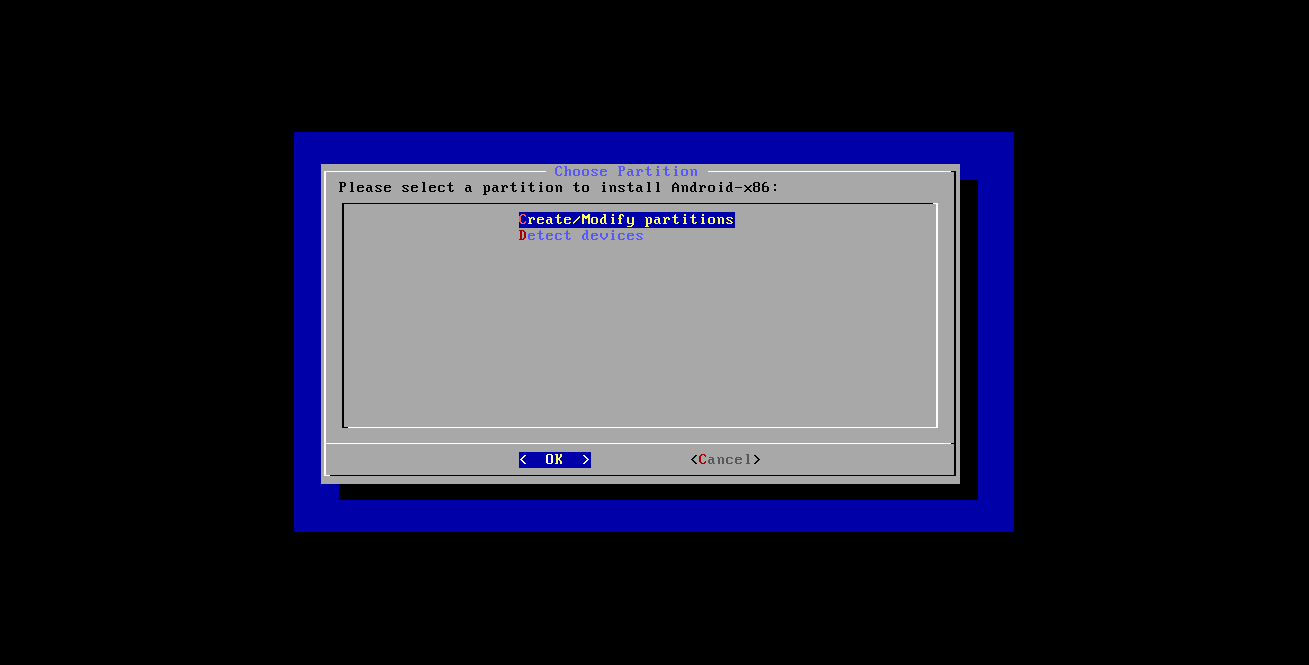
\includegraphics[width = 1\textwidth]{images/install2.png}
\end{figure}

در این مرحله اولین گزینه را انتخاب می‌کنیم. در صورتی که محیط نصب از ما پرسید که آیا قصد استفاده از GPT داریم یا نه، گزینه No را انتخاب می‌کنیم تا به محیط زیر برسیم:

\begin{figure}[ht]
	\centering	
	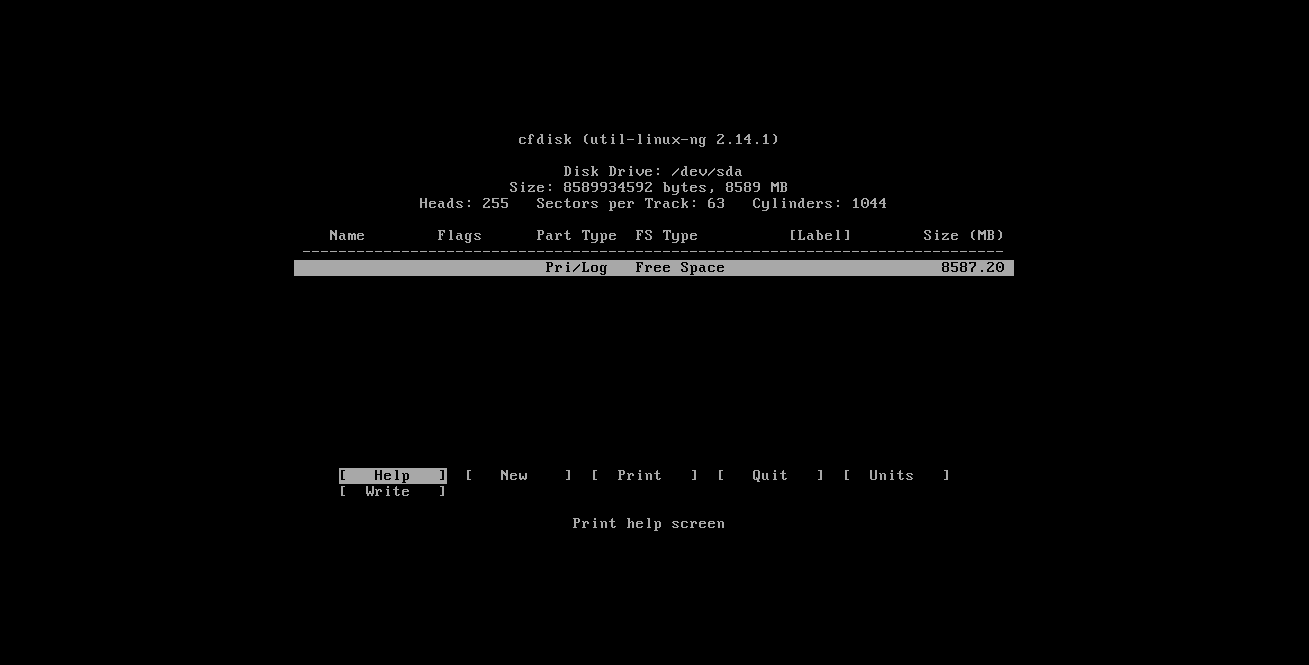
\includegraphics[width = 1\textwidth]{images/install3.png}
\end{figure}

در این جا بایستی پارتیشن‌بندی محیط اندرویدمان را انجام دهیم. همان‌طور که می‌بینید تنها همان ۸ گیگ حافظه درایو مجازی که قبل‌تر ساخته بودیم برای این کار در دسترس است، برای ساختن یک پارتیشن جدید گزینه New را انتخاب می‌کنیم. سپس سیستم این سؤال را از ما می‌پرسد:

\begin{figure}[ht]
	\centering	
	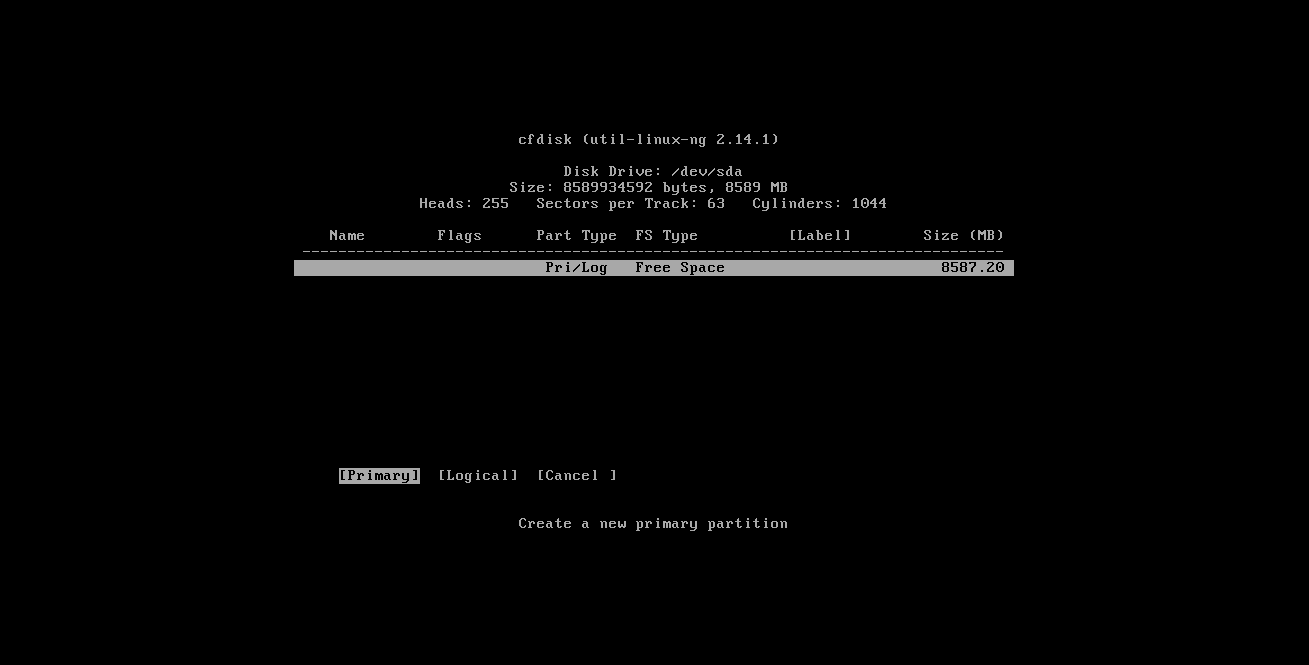
\includegraphics[width = 1\textwidth]{images/install4.png}
\end{figure}

همان‌طور که می‌بینید باید انتخاب کنیم که آیا پارتیشن ما Primary است یا Logical. ما گزینه Primary را انتخاب کرده و ادامه می‌دهیم:

\newpage

\begin{figure}[ht]
	\centering	
	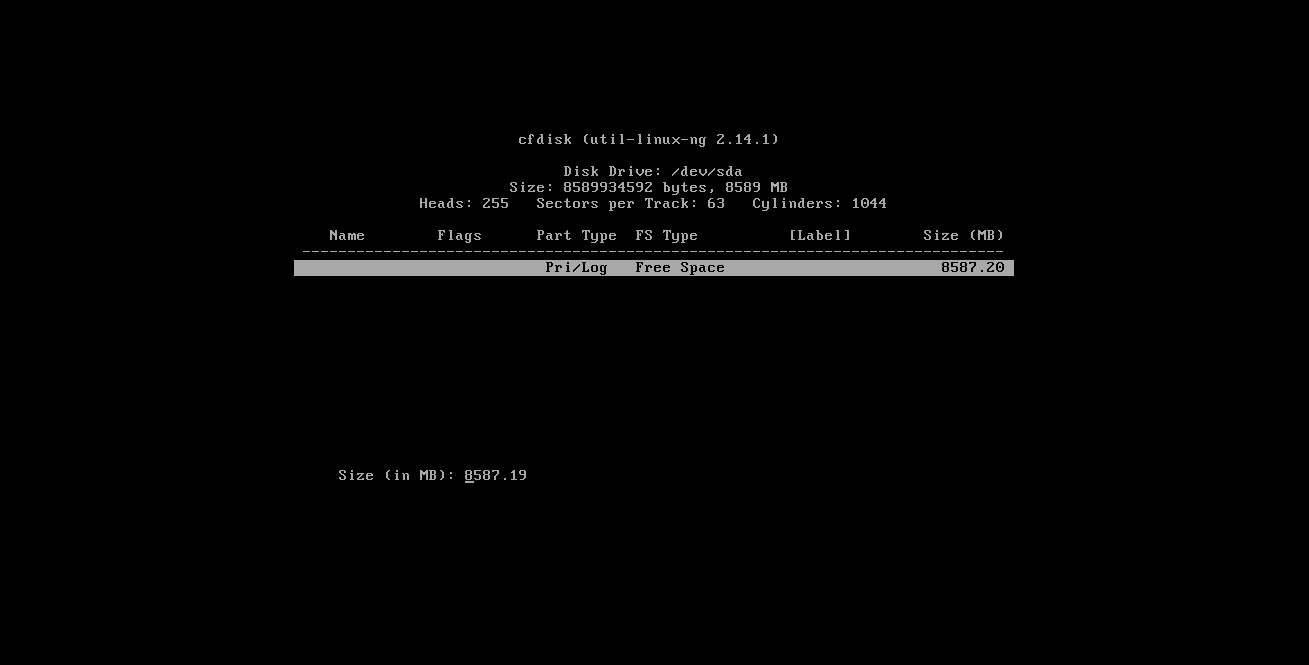
\includegraphics[width = 1\textwidth]{images/install5.png}
\end{figure}

در این جا محیط نصب میزان حافظه‌ای که ما می‌خواهیم را از ما می‌پرسد که بایستی مقداری کوچک‌تر یا مساوی مقدار حافظه درایو مجازی ما باشد. در صورتی که تغییری در این مقدار ایجاد نکنیم همان بیش‌ترین مقدار ممکن و کل درایو مجازی برای پارتیشن ما انتخاب می‌شود، ما نیز چنین می‌کنیم.

\begin{figure}[ht]
	\centering	
	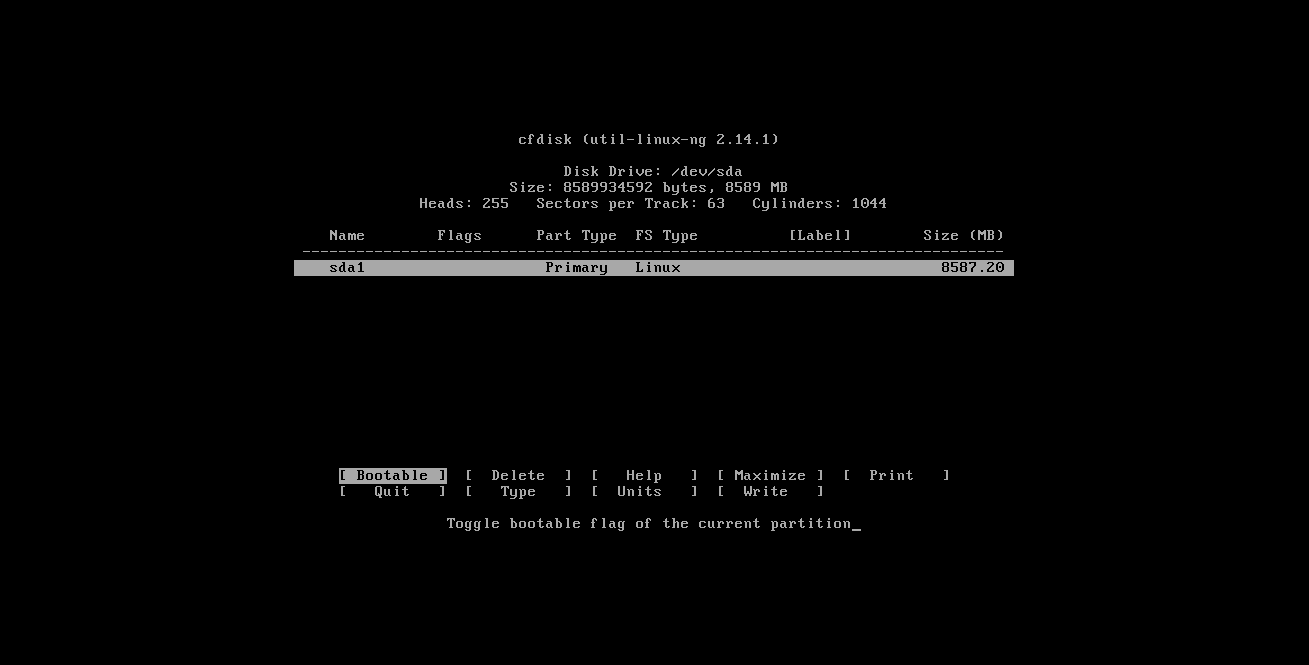
\includegraphics[width = 1\textwidth]{images/install6.png}
\end{figure}

سپس در این مرحله باید فلگ Bootable را به پارتیشن‌مان اضافه کنیم تا بتوان اندروید را روی آن بوت کرد، روی دکمه Bootable رفته و با فشردن دکمه Enter این کار را انجام می‌دهیم.

\newpage

\begin{figure}[ht]
	\centering	
	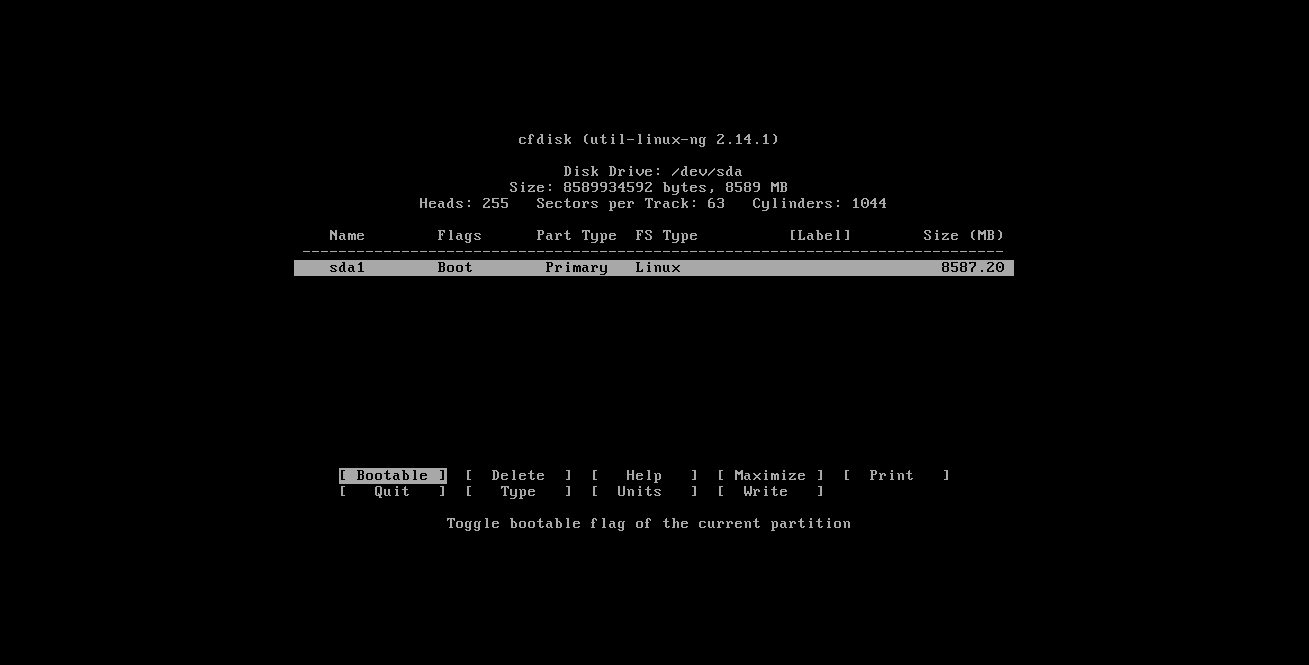
\includegraphics[width = 1\textwidth]{images/install7.png}
\end{figure}

پس از ظاهر شدن فلگ Boot جلوی پارتیشن مورد نظران روی گزینه Write رفته و با فشردن دکمه Enter تغییرات را روی آن اعمال می‌کنیم. ابتدا محیط نصب به شکل زیر و سپس به شکل زیر در می‌آید:

\begin{figure}[ht]
	\centering	
	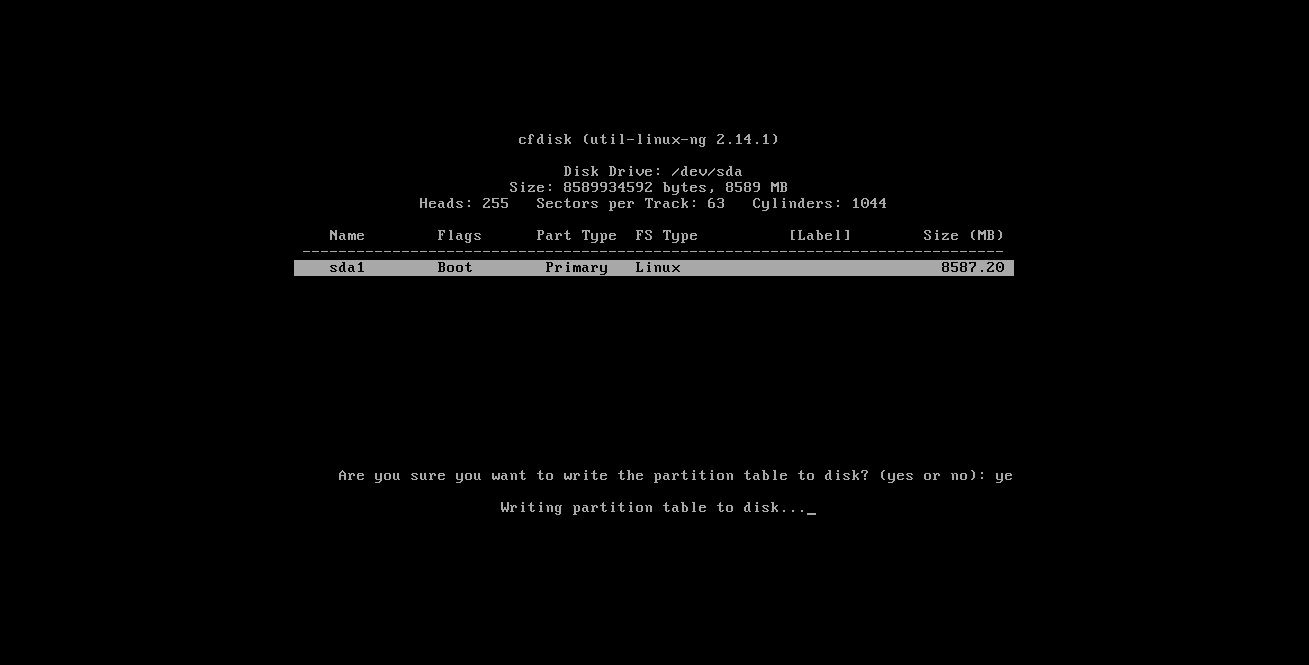
\includegraphics[width = 1\textwidth]{images/install8.png}
\end{figure}

\newpage

\begin{figure}[ht]
	\centering	
	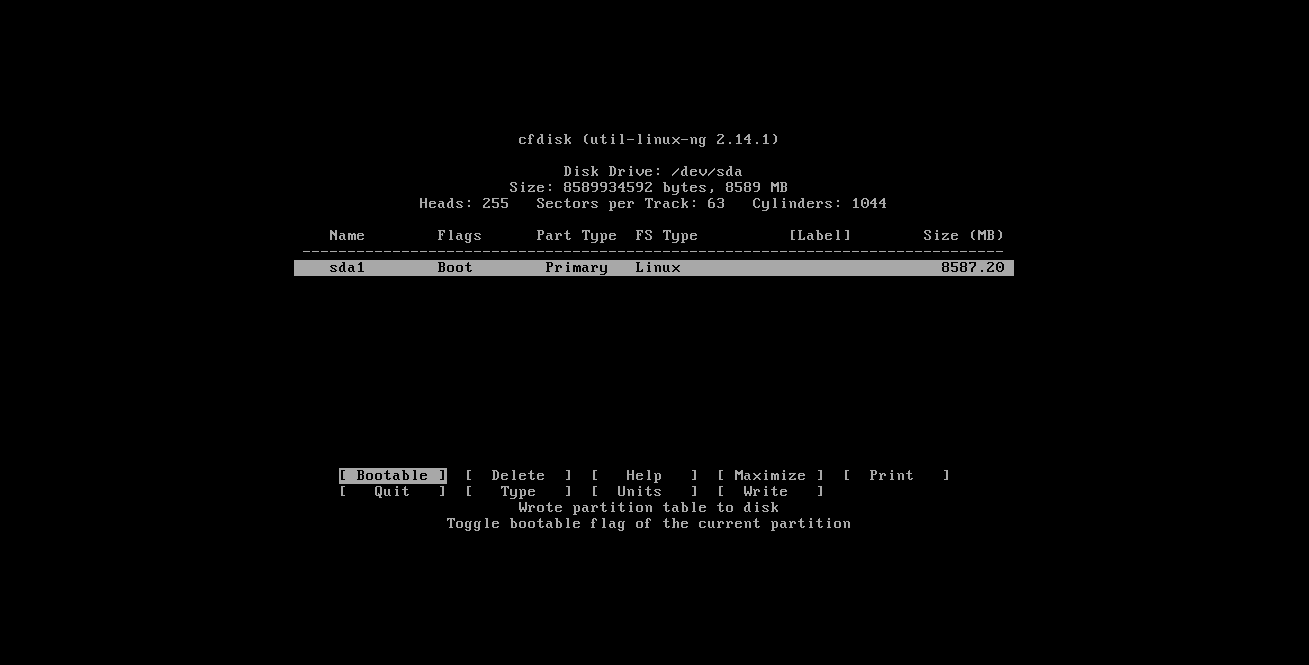
\includegraphics[width = 1\textwidth]{images/install9.png}
\end{figure}

سپس Quit را می‌زنیم تا به این محیط برگردیم:

\begin{figure}[ht]
	\centering	
	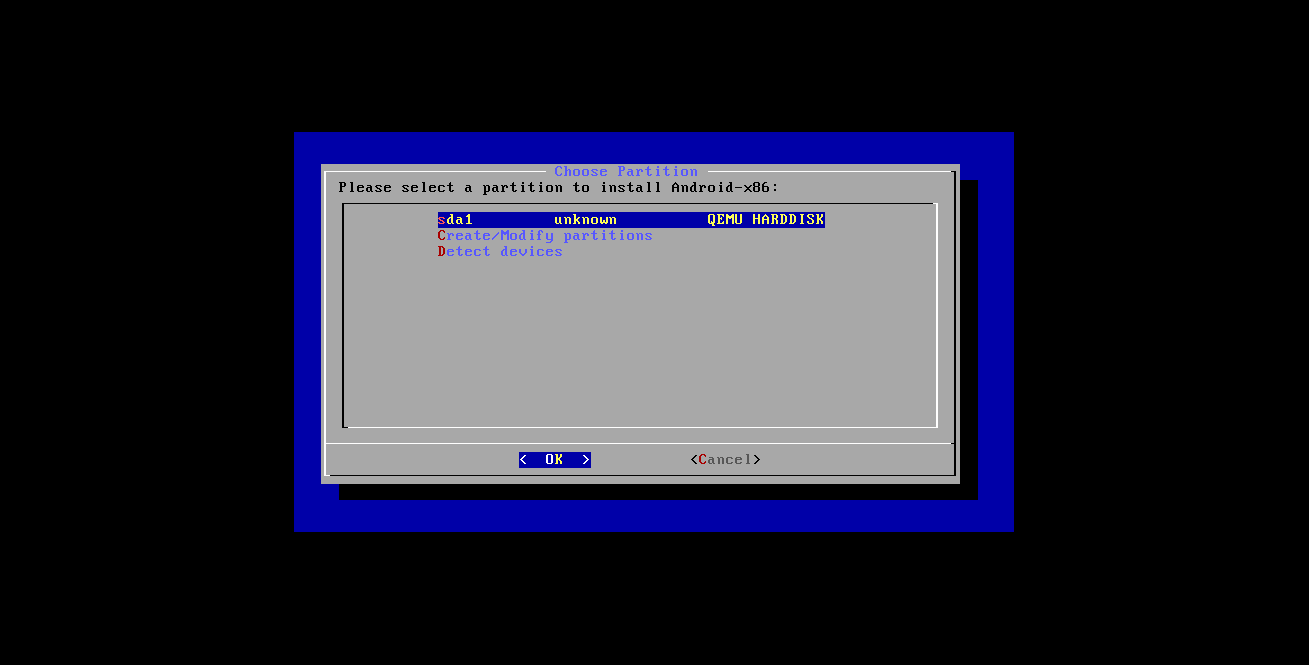
\includegraphics[width = 1\textwidth]{images/install10.png}
\end{figure}

در این جا پارتیشنی که در مراحل قبل درست‌ کرده‌ایم را می‌بینیم، حال باید نوع فایل‌سیستم آن را انتخاب کنیم. با فشردن دکمه Enter این کار را انجام می‌دهیم.

\begin{figure}[ht]
	\centering	
	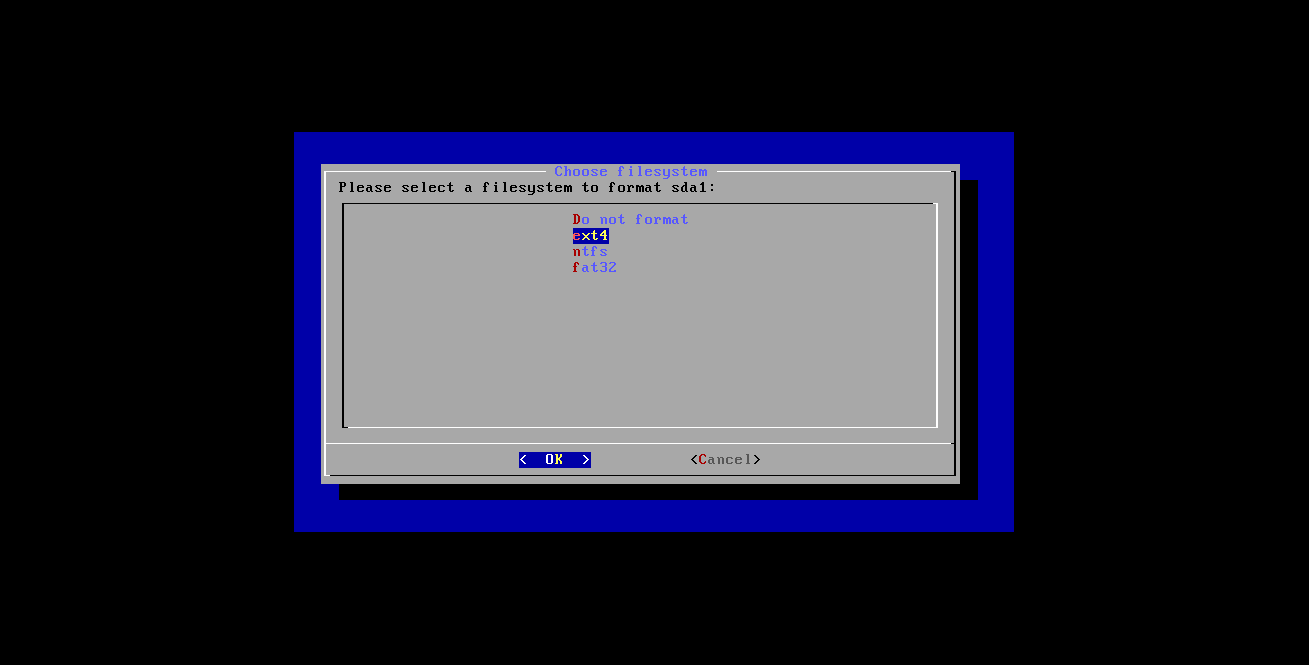
\includegraphics[width = 1\textwidth]{images/install11.png}
\end{figure}

\newpage

در این مرحله فایل‌سیستم ext4 را انتخاب می‌کنیم و در صورت پرسش مجدد آن را تایید می‌کنیم تا به این جا برسیم:

\begin{figure}[ht]
	\centering	
	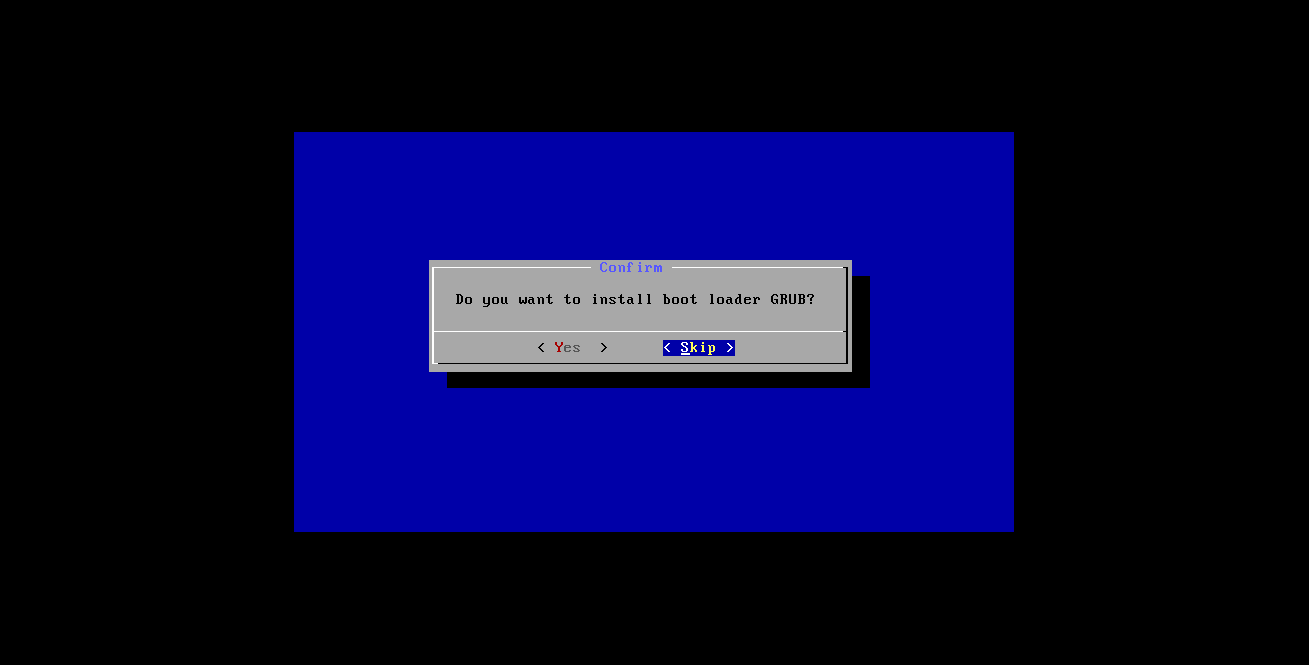
\includegraphics[width = 1\textwidth]{images/install12.png}
\end{figure}

در این مرحله نیز Yes را انتخاب می‌کنیم.

\newpage

\begin{figure}[ht]
	\centering	
	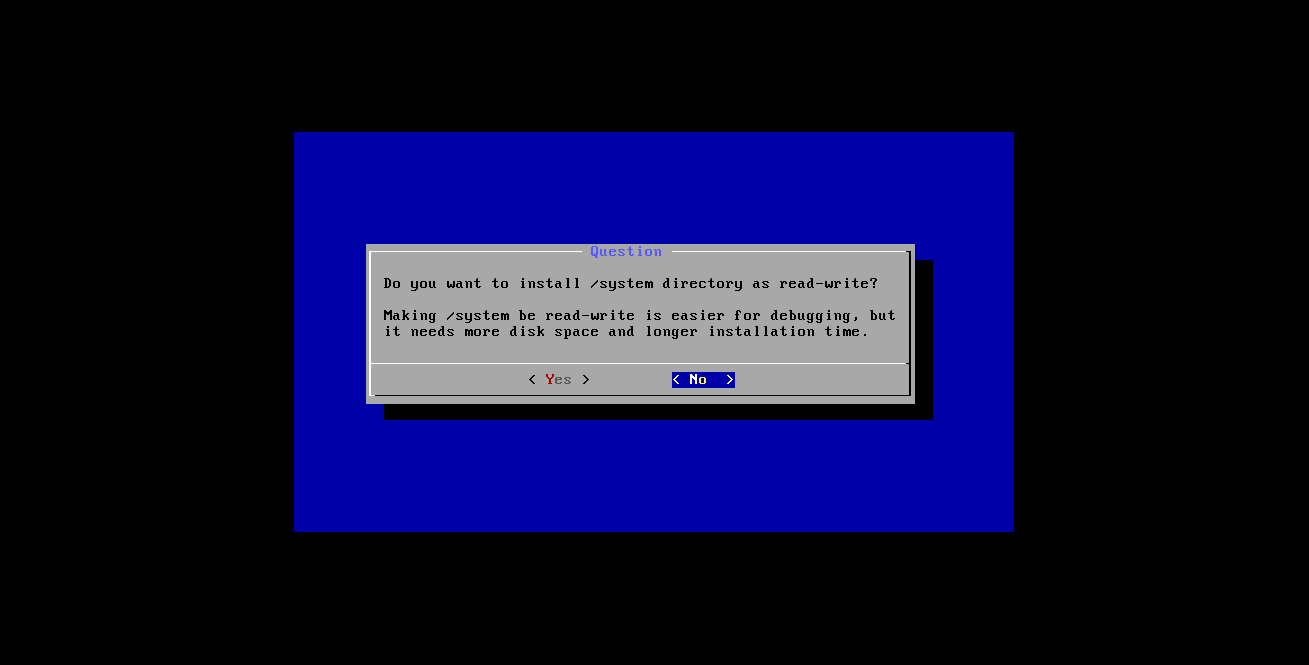
\includegraphics[width = 1\textwidth]{images/install13.png}
\end{figure}

در این جا محیط نصب از ما می‌پرسد که آیا قصد داریم دایرکتوری سیستم را با دسترسی read/write نصب کنیم یا نه که ما Yes را انتخاب می‌‌کنیم. سپس فرایند نصب شروع می‌شود:

\begin{figure}[ht]
	\centering	
	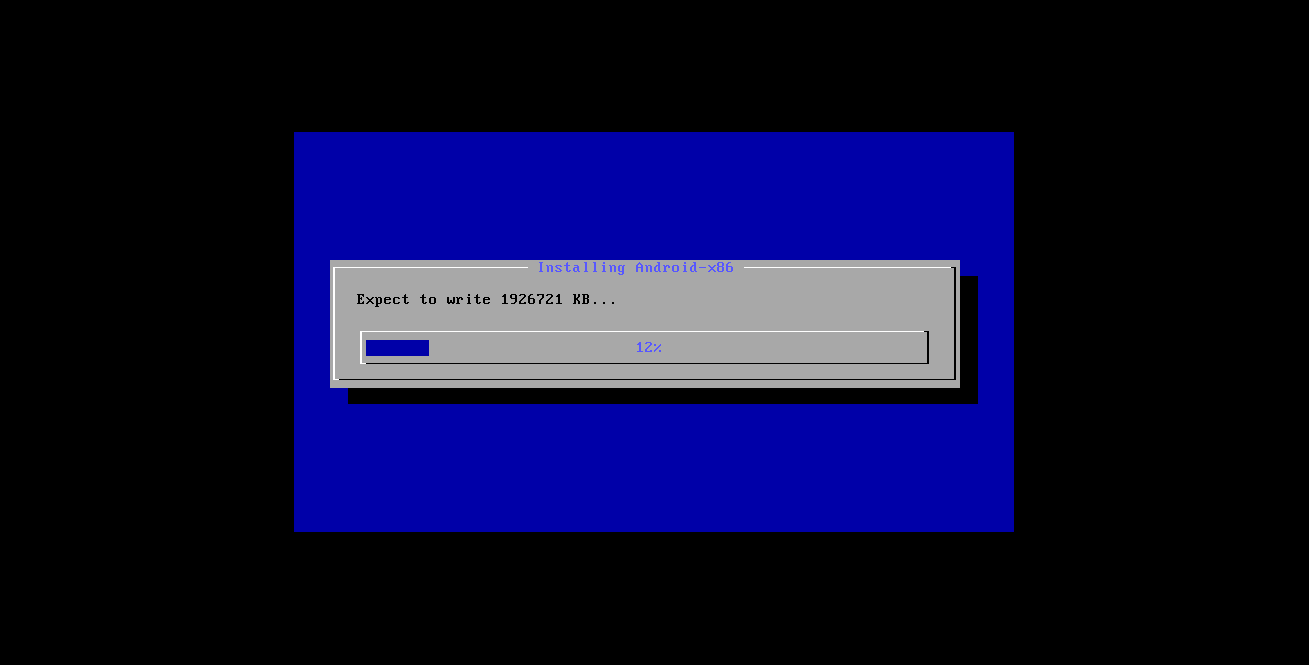
\includegraphics[width = 1\textwidth]{images/install14.png}
\end{figure}

اجازه می‌دهیم تا نصب تمام شود تا به این جا برسیم:

\newpage

\begin{figure}[h]
	\centering	
	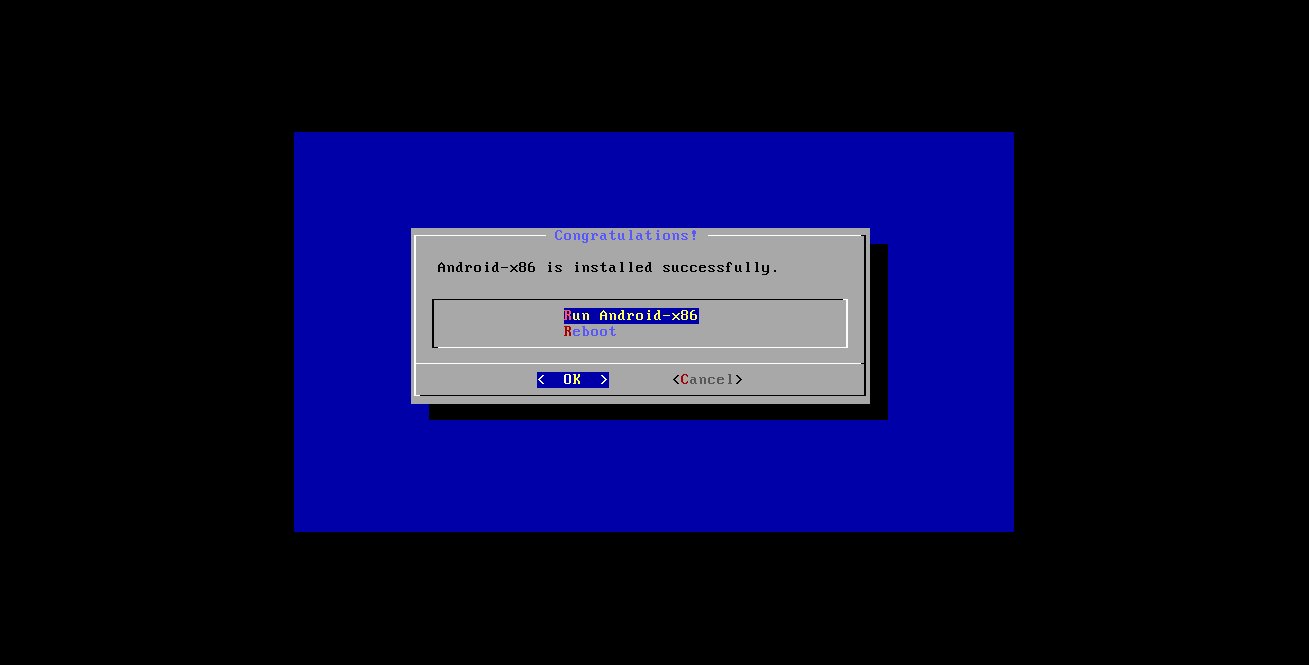
\includegraphics[width = 1\textwidth]{images/install15.png}
\end{figure}

در این جا می‌توانیم اندروید را اجرا کنیم، سیستم را Reboot کنیم یا حتی از سیستم خارج شویم، زیرا اندروید اکنون روی درایو مجازی ما نصب شده و می‌توانیم هر زمان که خواستیم آن را روی آن اجرا کنیم. از جایی که مرتبه قبل این کار را با VNC و Vinagre انجام دادیم این‌بار از خود QEMU استفاده می‌کنیم تا حالات مختلف را پوشش داده باشیم.

به این منظور اجرایی قبلی را متوقف کرده و دستور زیر را در دایرکتوری‌مان اجرا می کنیم:

\begin{latin}
\begin{verbatim}
$ qemu-system-x86_64 -m 2048 -boot d -enable-kvm \
-smp 3 -net nic -net user -hda android71.qcow2	
\end{verbatim}
\end{latin}

همان‌طور که می‌بینیم این‌بار در دستور ما خبری از استفاده از VNC برای نمایش خروجی و نیز آدرس فایل ایزو برای بوت کردن نیست، بلکه می‌دانیم که سیستم‌عاملمان روی درایو مجازی نصب شده و آن را از روی درایو مجازی‌مان بوت می‌کنیم.

محیط QEMU اجرا شده و با GRUB مواجه می‌شویم:

\begin{figure}[h]
	\centering	
	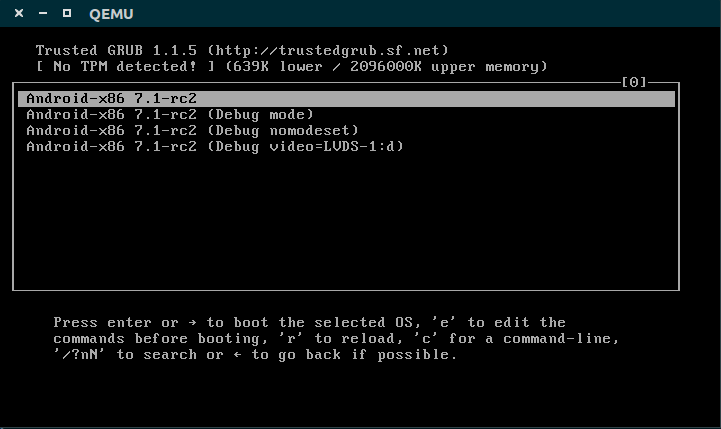
\includegraphics[width = 0.7\textwidth]{images/install16.png}
\end{figure}

گزینه اول را انتخاب می‌کنیم تا وارد سیستم اندروید شویم:

\newpage

\begin{figure}[h]
	\centering	
	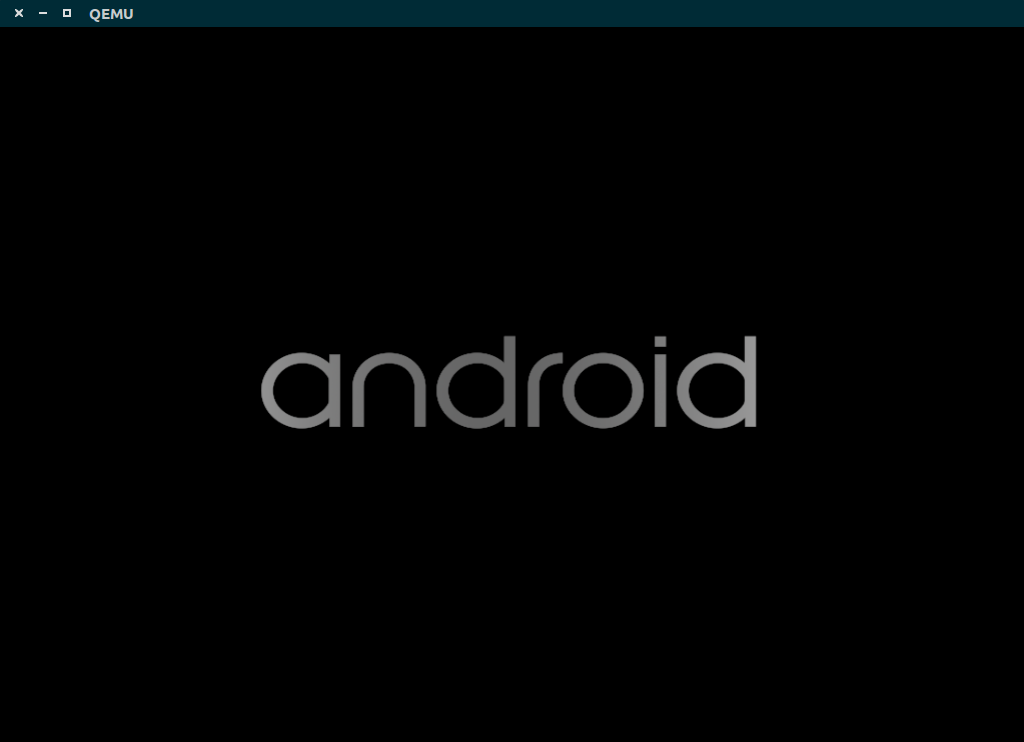
\includegraphics[width = 0.8\textwidth]{images/install18.png}
\end{figure}

با پدیدار شدن این نشان اندروید شروع به بوت شدن می‌کند. سپس محیط زیر پدیدار می‌شود:

\begin{figure}[h]
	\centering	
	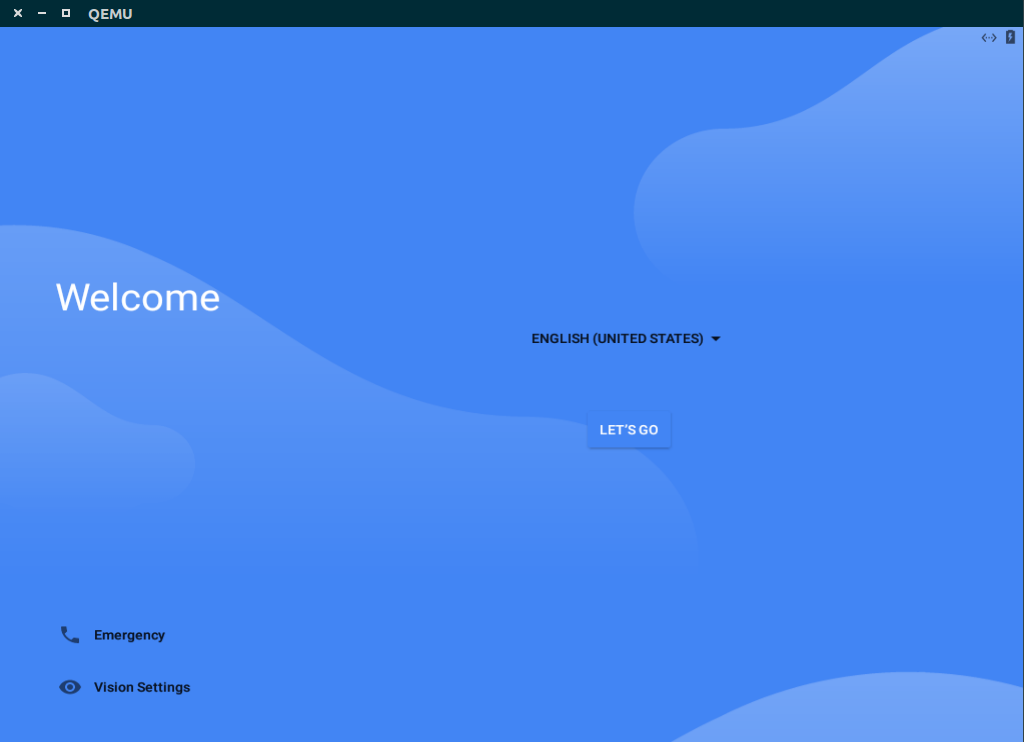
\includegraphics[width = 0.8\textwidth]{images/install19.png}
\end{figure}

مراحل را به ترتیب رد می‌کنیم تا به محیط کار اندروید برسیم(این مراحل به دلیل سادگی و طولانی بودن در این مستند آورده نشده‌اند):

\newpage

\begin{figure}[h]
	\centering	
	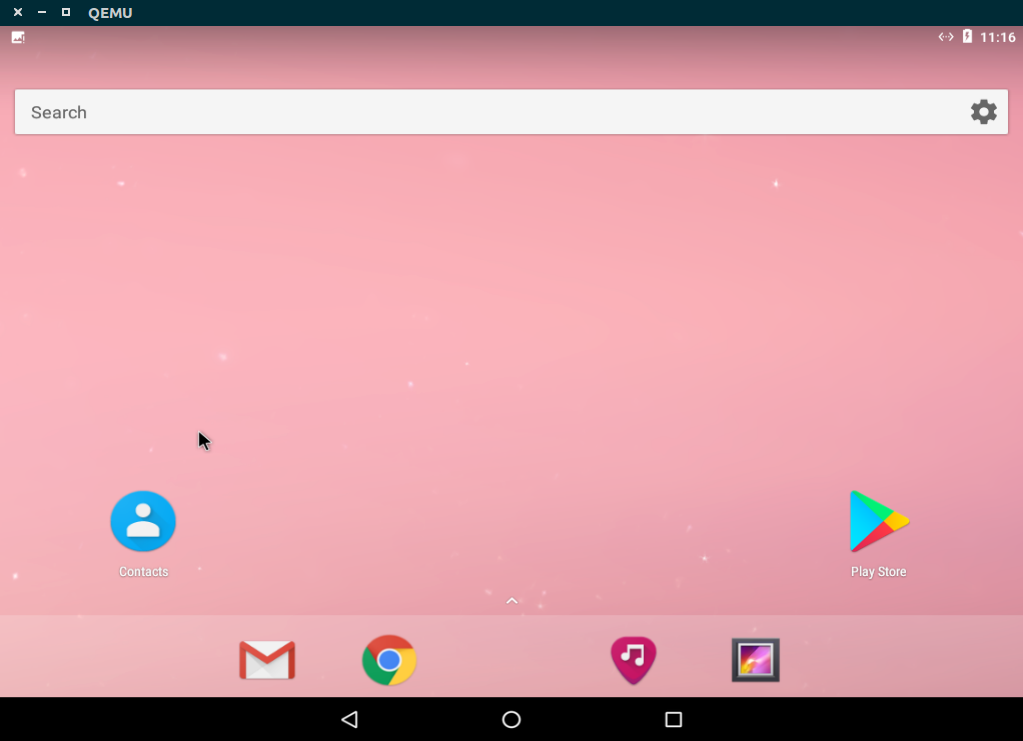
\includegraphics[width = 0.8\textwidth]{images/install20.png}
\end{figure}

برنامه‌ی terminal emulator به صورت پیش فرض روی این ماشین مجازی نصب بود. این برنامه را اجرا می‌کنیم:

\begin{figure}[h]
	\centering	
	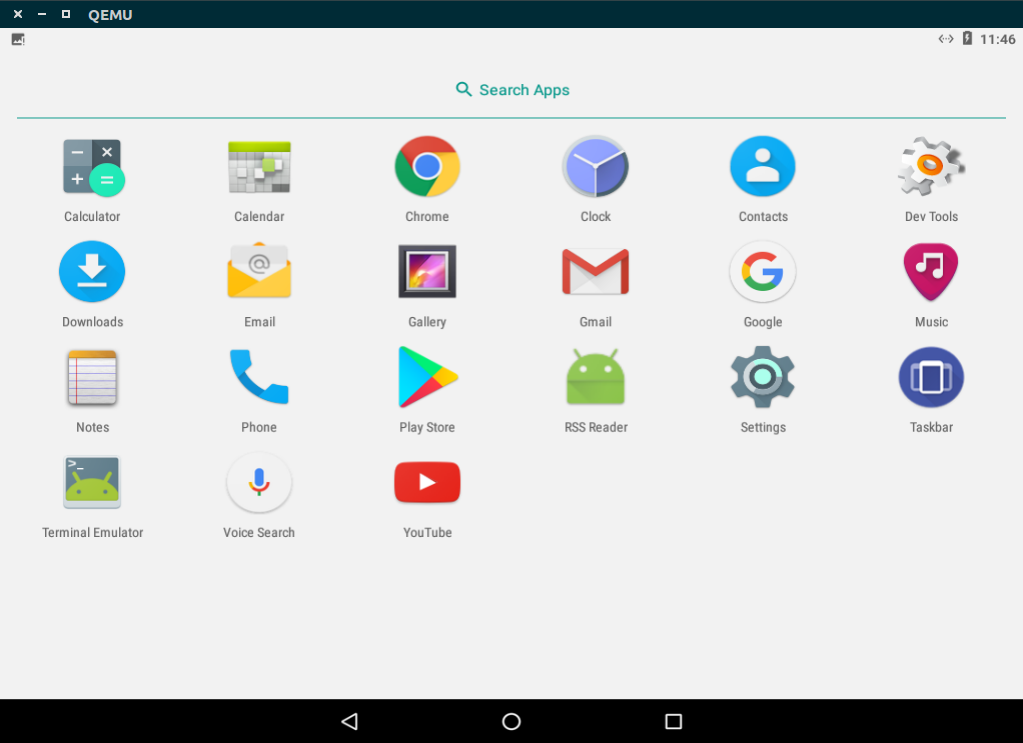
\includegraphics[width = 0.8\textwidth]{images/install21.png}
\end{figure}

با محیط زیر مواجه می‌شویم:

\newpage

\begin{figure}[h]
	\centering	
	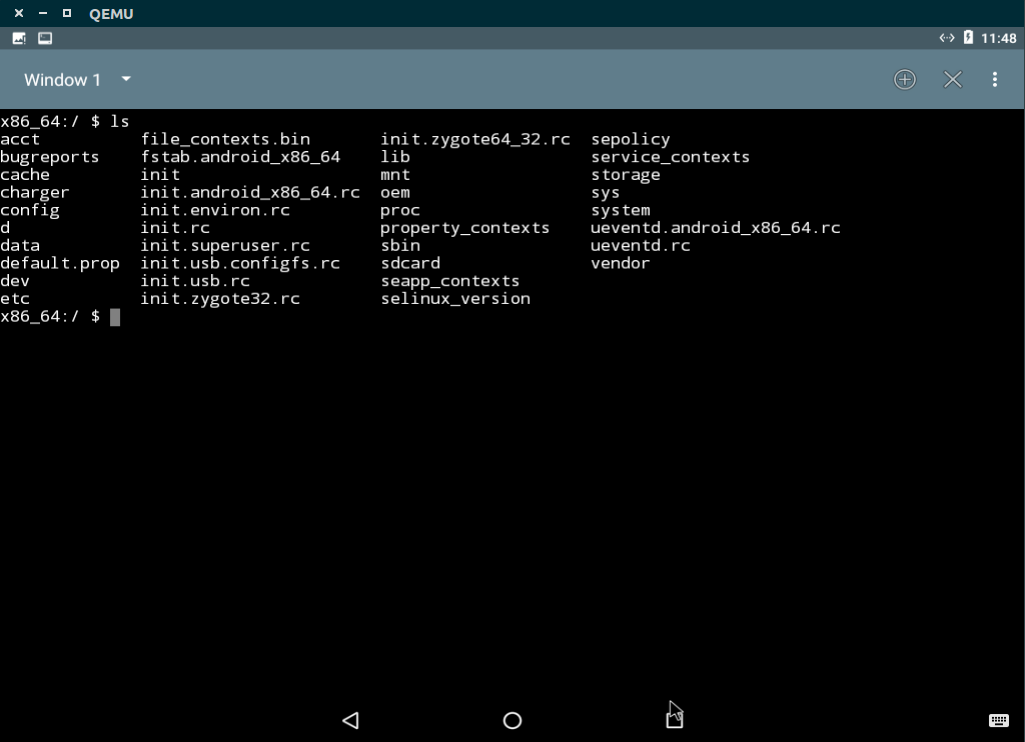
\includegraphics[width = 0.8\textwidth]{images/install22.png}
\end{figure}

\section*{اضافه کردن ابزار‌های مورد نیاز}

اولین چیزی که در محیط اندروید به آن نیاز داریم، یک برنامه شبیه‌ساز ترمینال است که به ما امکان مدیریت پکیج‌های موجود روی محیط اندروید است. برای مثال روی محیط فعلی اندروید کامپایلر C وجود ندارد.

به این منظور ابزار Termux را روی محیط نصب می‌‌کنیم.

\begin{figure}[h]
	\centering	
	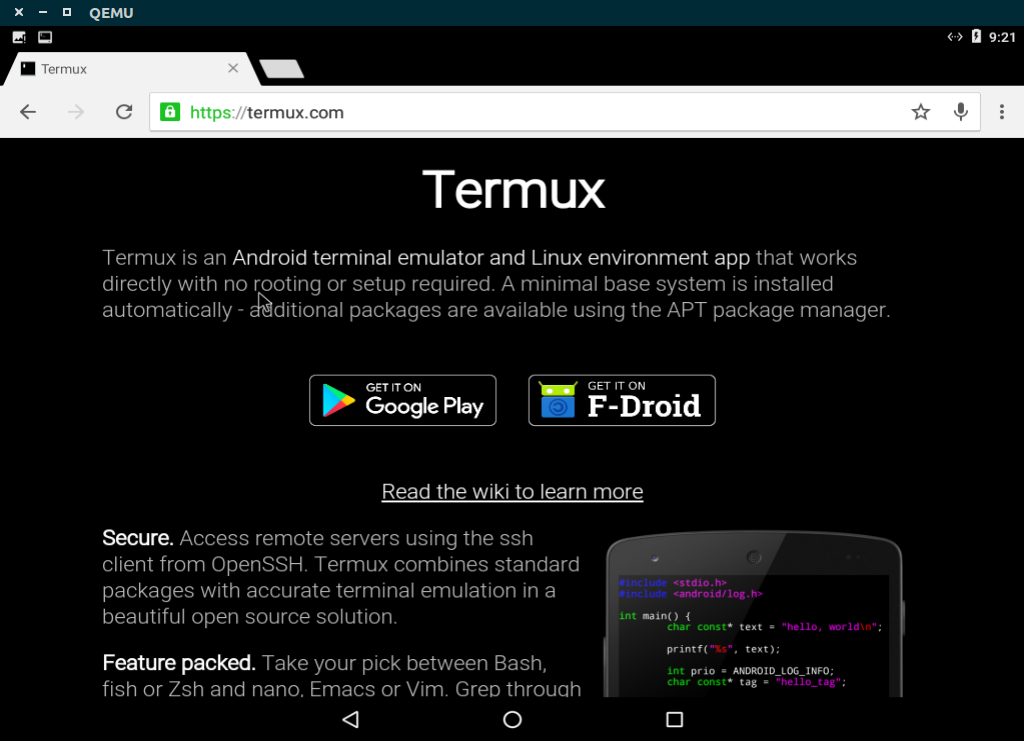
\includegraphics[width = 0.8\textwidth]{images/package1.png}
\end{figure}

این نرم‌افزار را از
\href{http://www.termux.com/}{سایت مرجع آن}
دریافت می‌کنیم. به این صفحه رفته و سپس گزینه دریافت از F-Droid را انتخاب می‌کنیم و در صفحه‌ای که باز می‌شود فایل apk برنامه را گرفته و نصب می‌کنیم. در حین فرایند نصب هر دسترسی که لازم بود به Termux می‌دهیم. در نهایت صفحه Termux مشابه زیر باز می‌شود:

\begin{figure}[h]
	\centering	
	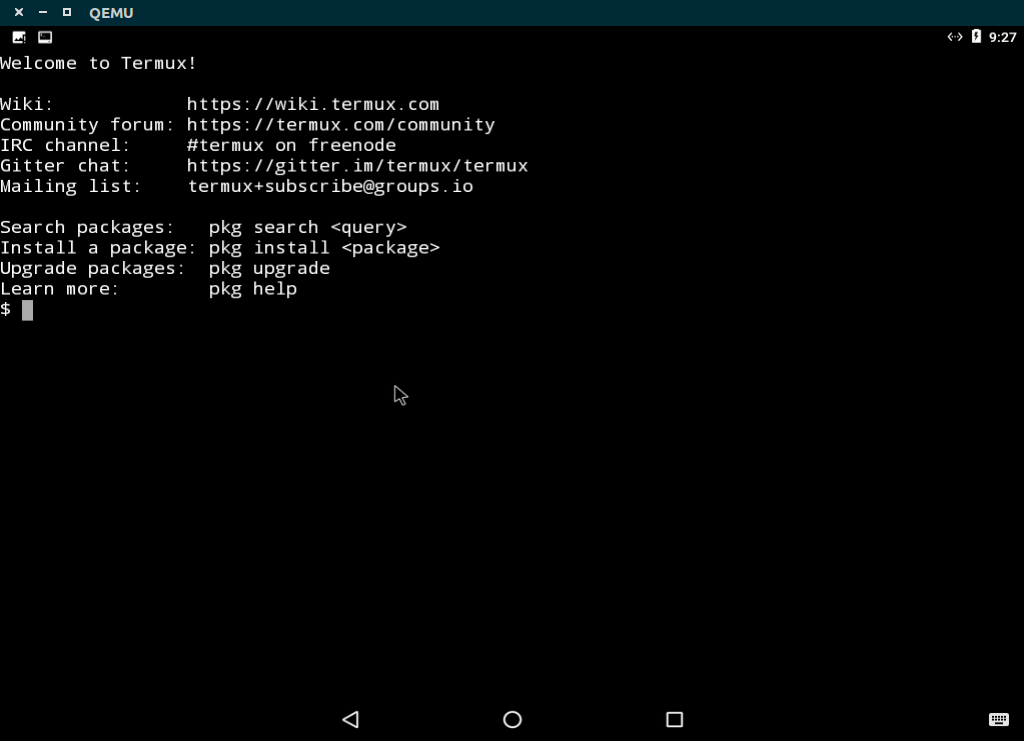
\includegraphics[width = 0.8\textwidth]{images/package5.png}
\end{figure}

در ادامه به منظور نصب پکیج‌های مورد نیاز apt را نصب و به‌روز‌رسانی می‌کنیم. این کار با این دستورهای زیر انجام می‌شود:

\begin{latin}
\begin{verbatim}
$ apt install
$ apt update
\end{verbatim}
\end{latin}

سپس پکیج‌هایی که در دستورات زیر آمده است را نصب می‌کنیم، در ادامه دلیل نصب هر کدام از این پکیج‌ها را ذکر می‌کنیم:

\begin{latin}
\begin{verbatim}
$ apt install tree
$ apt install git
$ apt install vim
$ apt install clang
$ apt install proot
$ apt install termux-tools
\end{verbatim}
\end{latin}

پکیج tree که برای پیمایش دایرکتوری‌ها در ترمینال استفاده می‌شود. از git نیز برای متصل شدن به مخزن git مان و فرستادن فایل‌های مد نظر به آن استفاده می‌کنیم. از vim نیز برای ویرایش فایل‌های متنی استفاده می‌کنیم. clang نوعی کامپایلر C است و از proot برای شبیه‌سازی ساختار root لینوکس در محل اجرای یک پردازه(مشخصا پردازه برنامه Termux ) استفاده می‌کنیم. termux-tools نیز برای افزودن برخی قابلیت‌ها به Termux استفاده می‌کنیم. سپس با دستور زیر پکیج‌های نصب‌شده را به‌روز می‌کنیم:

\begin{latin}
\begin{verbatim}
$ apt upgrade
\end{verbatim}
\end{latin}

سپس با دستور زیر فولدر‌های موجود در آدرس home ساختار یک سیستم عامل لینوکس را ذیل فولدر home برنامه Termux شبیه‌سازی می‌کنیم، برای مثال فولدر‌های Downloads ، Music و فولدر‌های دیگر.

\begin{latin}
\begin{verbatim}
$ termux-setup-storage
\end{verbatim}
\end{latin}

پس از وارد کردن این دستور برنامه Termux از سیستم عامل اندروید درخواست دسترسی می‌کند که با این درخواست موافقت می‌کنیم.

\begin{figure}[h]
	\centering	
	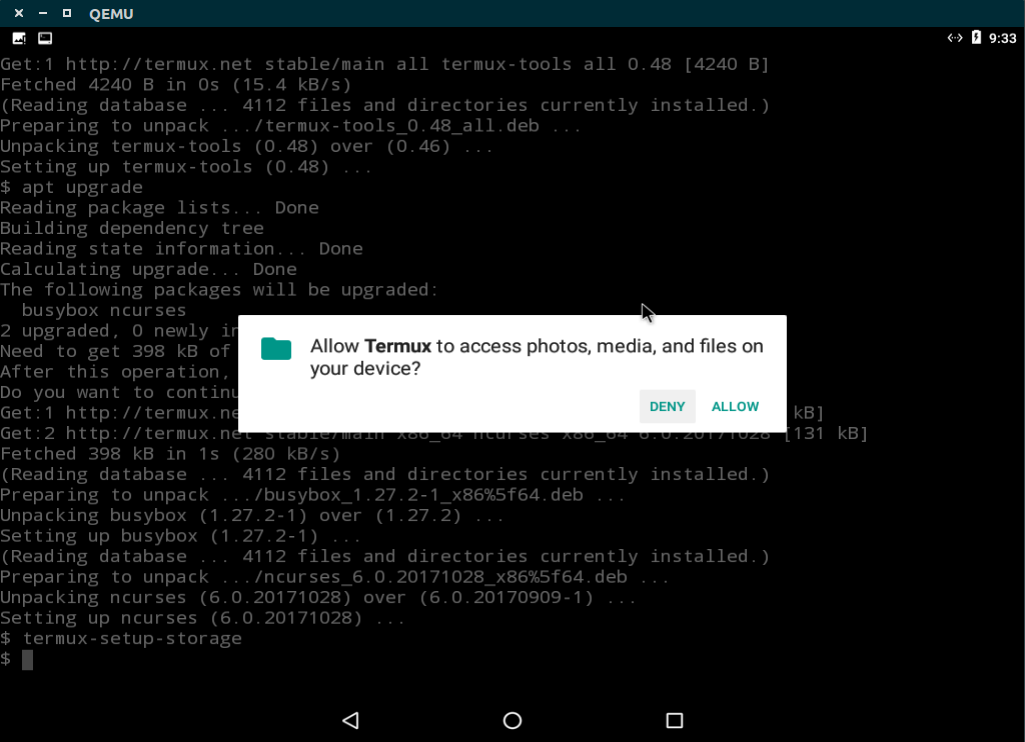
\includegraphics[width = 0.8\textwidth]{images/package6.png}
\end{figure}

سپس برای تنظیم محیط bash و vim به منظور تسهیل کار دو فایل .bashrc و .vimrc را در آدرس home ساخته و در هر کدام دستوراتی قرار می‌دهیم. در فایل .bashrc این دستورات:

\begin{latin}
\begin{verbatim}
clear
echo "Welcome! :"
PS1 = 'osprj@android:\w$'
\end{verbatim}
\end{latin}

و در فایل .vimrc این دستورات:

\begin{latin}
\begin{verbatim}
:syntax on
:set number
:set autoindent
\end{verbatim}
\end{latin}

\section*{اتصال به مخرن گیت}

به این منظور فولدری با نام VC در آدرس home ساخته و مخزن گیت‌مان را در آن جا clone می‌کنیم:

\begin{latin}
\begin{verbatim}
~$ mkdir VC
~$ cd VC
~/VC$ git clone https://github.com/faryabimm/OS_course_project_961.git
\end{verbatim}
\end{latin}

\section*{گرفتن خروجی دستور‌های logcat و dmesg}

به این منظور در دایرکتوری بالا فولدری با نام \lr{phase\_1} و ذیل آن فولدری با نام \lr{part\_1} برای انجام بخش اول این فاز یعنی گرفتن خروجی دستور‌های ذکر‌شده می‌سازیم. سپس به این دایرکتوی رفته و خروجی دستورات را به وسیله دستور‌های زیر ذخیره می‌کنیم:

\begin{latin}
\begin{verbatim}
$ logcat > logcat_all.txt
$ # because logcat is an open stream we need to manually terminate it
$ # <ctrl> + <c>
\end{verbatim}
\end{latin}

اما برای اجرای فراخوانی dmesg نیاز به دسترسی root داریم و باید از دستور su استفاده کنیم. دقت کنید که پس از این حالت به صورت خودکار به آدرس / سیستم منتقل می‌شویم و باید مجددا به آدرس home برنامه Termux که قبلا در آن بودیم برگردیم. پس از این کار دستور dmesg را مانند دستور قبل اجرا کرده و خروجی آن را در یک فایل متنی می‌ریزیم. همین‌طور باید دقت داشت از جایی که فایل متنی‌مان در حالت root ایجاد شده بایستی اجازه دسترسی به آن را به سایر کاربران نیز بدهیم.

\begin{latin}
\begin{verbatim}
$ su
# cd /data/data/com.termux/files/home/VC/OS_course_project_961/
  phase_1/part_1/
# dmesg > dmesg_all.txt
# chmod 777 dmesg.txt
# exit
\end{verbatim}
\end{latin}

حال با دستورات زیر ۵۰ خط آخر هر فایل را استخراج کرده و در یک فایل متنی جدید ذخیره می‌کنیم:

\begin{latin}
\begin{verbatim}
$ tail -50 logcat_all.txt > logcat_50.txt
$ tail -50 dmesg_all.txt > dmesg_50.txt
\end{verbatim}
\end{latin}

\section*{تحلیل خروجی دستور dmesg}
خروجی دستور dmesg حاوی اطلاعات تمامی اتفاقات رخ داده در سطح کرنل شامل گزارش‌های رخداد، خطا‌های ایجاد شده و هشدار‌های سیستمی است. هر خط در این فایل شامل بخش‌های مختلفی است. ابتدای هر خط  زمان ثبت آن خط آورده می‌شود.

اکثر خطوط این فایل خروجی‌های سیستم ثبت رخداد audit هستند. در این خطوط نوع سرویسی که یک پردازه درخواست کرده و از آن گرفته شده و سایر اطلاعات مربوط به پردازه و سرویس و کد خطا آورده می‌شود. خط زیر مثالی از این خطوط است:

\begin{latin}
\begin{verbatim}
[21100.340339] type=1400 audit(1509913800.012:1173):
avc: denied { setcurrent } for pid=6692 comm="main"
scontext=u:r:init:s0 tcontext=u:r:init:s0 tclass=process permissive=1
\end{verbatim}
\end{latin}

سایر خطوط این فایل شامل رخداد‌های تغییر فرکانس کلاک پردازه‌ی اصلی،

\begin{latin}
\begin{verbatim}
[ 9582.321072] clocksource: timekeeping watchdog on CPU1:
Marking clocksource 'tsc' as unstable because the skew is too large:
[ 9584.181099] clocksource:                       'hpet' wd_now:
b73075b5 wd_last: a3642ab8 mask: ffffffff
[ 9584.181099] clocksource:                       'tsc' cs_now:
143b7d2a281b cs_last: 143b3239a1c6 mask: ffffffffffffffff
[ 9585.138201] clocksource: Switched to clocksource hpet
\end{verbatim}
\end{latin}
اتمام پردازه‌های orphan و تحت قیومیت پردازه‌ی init
،
\begin{latin}
\begin{verbatim}
[22039.738638] init: Untracked pid 6815 exited with status 0
\end{verbatim}
\end{latin}

سیگنال‌های تولید شده و ارسال شده توسط کرنل،
\begin{latin}
\begin{verbatim}
[16510.788184] get_sys_time_ex[6492]: segfault at ac4e5c0 ip
00007b610ab8347b sp 00007ffe4cfff4a0 error 4 in libc.so[7b610ab55000+ea000]
\end{verbatim}
\end{latin}
خروجی‌های binder ،
\begin{latin}
\begin{verbatim}
[ 2823.744743] binder: undelivered transaction 377418, process died.
[ 2823.746074] binder: 1343:1343 transaction failed 29189/-22, size 100-0
line 2939
\end{verbatim}
\end{latin}
ثبت یک سخت افزار در سیستم،
\begin{latin}
\begin{verbatim}
[    5.521942] Registering sdcardfs 0.1
[    5.585714] input: ImExPS/2 Generic Explorer Mouse as
/devices/platform/i8042/serio1/input/input4
[   36.201087] input: Android Power Button as /devices/virtual/input/input5
\end{verbatim}
\end{latin}
و انواع دیگری از رخداد‌هاست.

فایل logcat یک امکان برای log گیری از پردازه‌های در حال اجرا در سیستم در \lr{user space} است. توسعه‌ دهندگان نرم افزار نیز می‌توانند با استفاده از مکانیزم‌های ارایه شده در کلاس‌های logging در زبان جاوا در این فایل به درج رکورد‌های مربوط به برنامه‌ی خود بپردازند و از آن برای دیباگ کردن برنامه استفاده کنند (مخصوصا در برنامه‌های چند ریسه‌ای امروزی که عملیات دیباگ بسیار پیچیده تر و سخت تر از برنامه‌های تک ریسه‌ایست).

در رکورد‌های این فایل زمان ثبت رخداد، pid ثبت کننده‌ی رکورد، pid پردازه‌ی هدف، نوع رکورد (
\lr{I: Information}
،
\lr{W: Warning}

\lr{E: Error}
)
، نام صادر کننده‌ی رکورد (به عنوان مثال AndroidRuntime یا SoundPool یا (APM\_AudioPolicyManager و اطلاعات پیام ذکر می‌شود.

در اینجا یک رکورد را به عنوان مثال آورده‌ایم:
\begin{latin}
\begin{verbatim}
11-06 00:15:53.401  1343  1415 E TaskPersister:
File error accessing recents directory (directory doesn't exist?).
\end{verbatim}
\end{latin}



\section*{پیاده‌سازی فراخوانی‌های سیستمی مورد نظر}

ابتدا به فولدر \lr{phase\_1} برگشته و فولدری جدید با نام \lr{part\_2} برای ذخیره‌سازی فایل‌ فراخوانی‌ های سیستمی ذکر‌شده ایجاد می‌کنیم و ذیل آن یک فولدر با نام time\_syscall و یک فولدر با نام cpu\_utilization\_syscall ، هر کدام برای دحیره‌سازی یک فراخوانی سیستمی. کد هر یک از این فراخوانی‌های سیستمی در مخزن پروژه موجود است.

خروجی نوعی این فراخوانی‌‌های سیستمی در عکس‌های زیر آمده است:

\begin{figure}[h]
	\centering	
	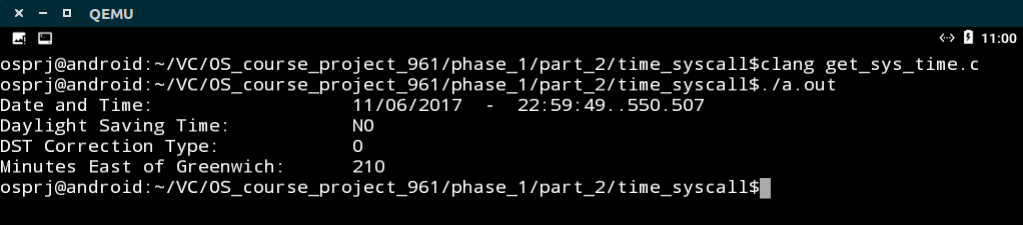
\includegraphics[width = 1\textwidth]{images/syscall1.png}
\end{figure}

\begin{figure}[h]
	\centering	
	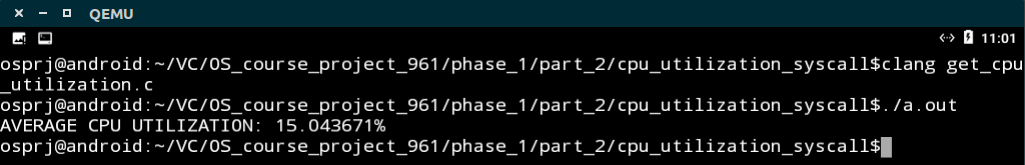
\includegraphics[width = 1\textwidth]{images/syscall2.png}
\end{figure}

\begin{thebibliography}{9}

\latin
\bibitem{1}
\url{https://www.qemu.org/}
\bibitem{2}
\url{https://en.wikipedia.org/wiki/Virtual_Network_Computing}
\bibitem{3}
\url{https://github.com/novnc/noVNC}
\bibitem{4}
\url{https://wiki.gnome.org/Apps/Vinagre}
\bibitem{5}
\url{https://en.wikipedia.org/wiki/Telnet}
\bibitem{6}
\url{https://fosspost.org/tutorials/install-android-6-0-marshmallow-linux-run-apps-games}
\end{thebibliography}

\end{document}